%Jennifer Pan, August 2011

\documentclass[10pt,letter]{article}
	% basic article document class
	% use percent signs to make comments to yourself -- they will not show up.

\usepackage{amsmath}
\usepackage{amssymb}
	% packages that allow mathematical formatting

\usepackage[final]{graphicx}
\usepackage{subcaption}
	% package that allows you to include graphics
\usepackage{tikz}
\usepackage{setspace}
	% package that allows you to change spacing

\onehalfspacing
	% text become 1.5 spaced

\usepackage{fullpage}
	% package that specifies normal margins

\renewcommand{\vector}[1]{\boldsymbol{#1}}
\newcommand{\problem}[1]{\section*{Problem #1}}
\newcommand{\problempart}[1]{\paragraph{#1}}

\begin{document}
	% line of code telling latex that your document is beginning


\title{ECON 511 Problem Set 3}

\author{Nicholas Wu}

\date{Spring 2021}
	% Note: when you omit this command, the current dateis automatically included

\maketitle
	% tells latex to follow your header (e.g., title, author) commands.
%\textbf{Note:} I use bold symbols to denote vectors and nonbolded symbols to denote scalars. I primarily use vector notation to shorthand some of the sums, since many of the sums are dot products.

\problem{1}
\problempart{(1)} This follows from Jensen's inequality. Since $1/x$ is convex,
\[ h \ge \frac{1}{\mu} \]
\problempart{(2)} The value of the expected PDV is
\[ V_{j,t} = \mathbb{E}_t \left( \sum_{s=1}^\infty \beta^s \frac{u'(c_{t+s})}{u'(c_t)}\pi_{j,t+s} \right) \]
The bond price is
\[ p^B_{j,t} = \mathbb{E}_t\sum_{s=1}^\infty \beta^s \frac{u'(c_{t+s})}{u'(c_t)} r \]
\[ = \sum_{s=1}^\infty \beta^s r \mathbb{E}_t \frac{u'(c_{t+s})}{u'(c_t)} \]
\[ = \sum_{s=1}^\infty \beta^s r \mathbb{E}_t \frac{c_t}{u'(c_{t+s})} \]
\[ = r c_t \sum_{s=1}^\infty \beta^s \mathbb{E}_t \frac{1}{u'(c_{t+s})} \]
\[ = r \pi_{j,t} \sum_{s=1}^\infty \beta^s h \]
\[ = \frac{r \pi_{j,t} \beta h}{1-\beta} \]
The stock price is
\[ p^N_{j,t} = \mathbb{E}_t\sum_{s=1}^\infty \beta^s \frac{u'(c_{t+s})}{u'(c_t)} \frac{\pi_{j,t+s} - rB}{N} \]
\[ = \sum_{s=1}^\infty \beta^s \mathbb{E}_t \frac{c_{j,t}}{c_{j,t+s}}\frac{\pi_{j,t+s} - rB}{N} \]
\[ = \sum_{s=1}^\infty \beta^s \pi_{j,t}\mathbb{E}_t \frac{\pi_{j,t+s} - rB}{N\pi_{j,t+s}}  \]
\[ = \sum_{s=1}^\infty \beta^s \pi_{j,t}\frac{1}{N}\mathbb{E}_t \left(1 - \frac{rB}{\pi_{j, t+s}} \right) \]
\[ = \sum_{s=1}^\infty \beta^s \pi_{j,t}\frac{1}{N} \left(1 - rBh \right) \]
\[ = \frac{\beta}{1-\beta} \pi_{j,t}\frac{1}{N} \left(1 - rBh \right) \]
\[ = \frac{\beta \pi_{j,t}\left(1 - rBh \right)}{N(1-\beta)}  \]
The asset prices and value of the firm are independent of time since cash flows are independent across periods, hence no information about the future is obtainable from the past. Hence the the asset prices and firm value don't depend on $t$.
\problempart{(3)}
\[ V_{j,t} = \mathbb{E}_t \left( \sum_{s=1}^\infty \beta^s \frac{u'(c_{t+s})}{u'(c_t)}\pi_{j,t+s} \right) \]
\[  = \mathbb{E}_t \left( \sum_{s=1}^\infty \beta^s \frac{\pi_{j,t}}{\pi_{j,t+s}}\pi_{j,t+s} \right) \]

\[  = \pi_{j,t} \sum_{s=1}^\infty \beta^s\]
\[ = \frac{\beta\pi_{j,t}}{1-\beta} \]
Now,
\[ p^B_{j,t} B + p^N_{j,t} N = \frac{r \pi_{j,t} \beta h B}{1-\beta} + \frac{\beta \pi_{j,t}\left(1 - rBh \right)}{1-\beta} \]
\[= \frac{\beta \pi_{j, t} }{1-\beta}(rhB + (1-rBh)) = \frac{\beta \pi_{j, t} }{1-\beta} = V_{j,t} \]
The stock price is decreasing in all three; the higher the rate or the more bonds issued, the less residual profits and hence lower the stock price. If more shares issued, there are fewer residual profits per share, and hence the stock price deceases.

\problempart{(4)}
For $V$:
\[ \mathbb{E}_t \left( \frac{V_{t+1}}{V_t} \mid \pi_t = \pi_j \right) = \mathbb{E}_t \left( \frac{\frac{\beta\pi_{j,t+1}}{1-\beta}}{\frac{\beta\pi_{j,t}}{1-\beta}} \mid \pi_t = \pi_j \right)  \]
\[ =  \mathbb{E}_t \left( \frac{\pi_{j,t+1}}{\pi_{j,t}} \mid \pi_t = \pi_j \right) \]
\[ =  \mathbb{E}_t \left( \frac{\pi_{t+1}}{\pi_{t}} \mid \pi_t = \pi_j \right) \]
\[ =  \mathbb{E}_t \left( \frac{\pi_{t+1}}{\pi_j} \mid \pi_t = \pi_j \right) \]
\[ =  \frac{\mathbb{E}_t \left( \pi_{t+1} \mid \pi_t = \pi_j \right)}{\pi_j} \]
\[ =  \frac{\mu}{\pi_j} \]
For $p^B$:

\[ \mathbb{E}_t \left( \frac{p^B_{t+1}}{p^B_t} \mid \pi_t = \pi_j \right) = \mathbb{E}_t \left( \frac{\frac{\beta r h \pi_{j,t+1}}{1-\beta}}{\frac{\beta r h \pi_{j,t}}{1-\beta}} \mid \pi_t = \pi_j \right)  \]
\[ =  \mathbb{E}_t \left( \frac{\pi_{j,t+1}}{\pi_{j,t}} \mid \pi_t = \pi_j \right) \]
\[ =  \mathbb{E}_t \left( \frac{\pi_{t+1}}{\pi_{t}} \mid \pi_t = \pi_j \right) \]
\[ =  \frac{\mu}{\pi_j} \]
For $p^N$:

\[ \mathbb{E}_t \left( \frac{p^N_{t+1}}{p^N_t} \mid \pi_t = \pi_j \right) = \mathbb{E}_t \left( \frac{\frac{\beta \pi_{j,t+1}(1-rBh)}{N(1-\beta)}}{\frac{\beta \pi_{j,t}(1-rBh)}{N(1-\beta)}} \mid \pi_t = \pi_j \right)  \]
\[ =  \mathbb{E}_t \left( \frac{\pi_{j,t+1}}{\pi_{j,t}} \mid \pi_t = \pi_j \right) \]
\[ =  \mathbb{E}_t \left( \frac{\pi_{t+1}}{\pi_{t}} \mid \pi_t = \pi_j \right) \]
\[ =  \frac{\mu}{\pi_j} \]
\problempart{(5)}
The expected rate of return on stock share is:
\[ \mathbb{E}_t \left(\frac{p^N_{t+1} + \frac{\pi_{t+1} - rB}{N}}{p^N_t} \right) = \mathbb{E}_t\left(\frac{p^N_{t+1} }{p^N_t}\right) + \mathbb{E}_t \left( \frac{\pi_{t+1} - rB}{N p^N_t} \right) \]
\[ = \frac{\mu}{\pi_j} + \mathbb{E}_t \left( \frac{\pi_{t+1} - rB}{\frac{\beta \pi_{j}(1-rBh)}{(1-\beta)}} \right)  \]
\[ = \frac{\mu}{\pi_j} + \frac{(1-\beta)}{\beta(1-rBh)}\mathbb{E}_t \left( \frac{\pi_{t+1} - rB}{\pi_{j}} \right)  \]
\[ = \frac{\mu}{\pi_j} + \frac{(1-\beta)}{\beta(1-rBh)}\left( \frac{\mu - rB}{\pi_{j}} \right)  \]
\[ = \frac{\mu}{\pi_j} + \frac{(1-\beta)}{\beta(1-rBh)}\left( \frac{\mu - rB}{\pi_{j}} \right)  \]
\[ = \frac{\mu}{\pi_j} + \frac{\mu - rB}{\frac{\beta \pi_j}{1-\beta}(1-rBh)} \]
\[ = \frac{\mu}{\pi_j} + \frac{r (\mu h - r B h)}{\frac{\beta r h \pi_j}{1-\beta}(1-rBh)} \]
\[ = \frac{\mu}{\pi_j} + \frac{r (\mu h - r B h)}{p^B_{t}(1-rBh)} \]
\[ = \frac{\mu}{\pi_j} + \frac{r}{p^B_t}\left( \frac{ \mu h - r B h}{1-rBh} \right) \]
From part 1, we know that $h \ge 1/\mu$, and hence $\mu h \ge 1$. Therefore
\[\left( \frac{ \mu h - r B h}{1-rBh} \right) \ge 1 \]
so
\[ \frac{\mu}{\pi_j} + \frac{r}{p^B_t}\left( \frac{ \mu h - r B h}{1-rBh} \right)\ge  \frac{\mu}{\pi_j} + \frac{r}{p^B_t}\]
Hence the expected return on stocks is more than the expected return on bonds
Additionally,
\[ \frac{\mu}{\pi_j} + \frac{r}{p^B_t}\left( \frac{ \mu h - r B h}{1-rBh} \right) \]
\[ = \frac{\mu}{\pi_j} + \frac{r}{p^B_t}\left( \frac{ \mu h - 1}{1-rBh} + 1 \right) \]
Hence increasing $rB$ decreases the denominator and increases the expected return on stocks.

The expected rate of return on stock is higher; the consumers are risk averse and hence need to be compensated for the uncertainty in returns. The expected return is increasing in $rB$; the more leveraged the firm is, the higher variance in the yield, and hence the riskier stocks are and the higher return is needed to compensate risk averseness.

\problem{2}
\problempart{(1)}
For (i.b),
\[ V(k,z) = \max \left[ \max_{k'} \left[(1-P)(zk^\theta - Rk)+ \beta E_{z'}V(k',z') \right], zk^\theta - Rk + \beta E_{z'}V((1-\delta)k, z') \right] \]
For (ii.a),
\[ V(k,z) = \max \left[ \max_{k'} \left[z(k')^\theta - Rk' - F + \beta E_{z'}V((1-\delta)k',z') \right], zk^\theta - Rk + \beta E_{z'}V((1-\delta)k, z') \right] \]
For (ii.b),
\[ V(k,z) = \max \left[ \max_{k'} \left[(1-P)(z(k')^\theta - Rk') + \beta E_{z'}V((1-\delta)k',z') \right], zk^\theta - Rk + \beta E_{z'}V((1-\delta)k, z') \right] \]
The $P$ model is probably more empirically relevant, since it can be interpreted as firms sacrificing some of their productivity for investment, rather than everyone having identical adjustment costs irrespective of firm size.

As for timing, in (i) the investment decision only impacts the future value of the firm, where as in (ii) it affects both the current value of capital and the future value.

As we stated earlier, the fixed adjustment cost $F$ is fixed regardless of productivity, where as the fractional cost $P$ may vary depending on productivity.
\problempart{(2)}
See code.
\problempart{(3)} See figure 1 for the benchmark graphs of the inaction bands.
\begin{center}
\begin{figure}
\begin{subfigure}{.5\textwidth}
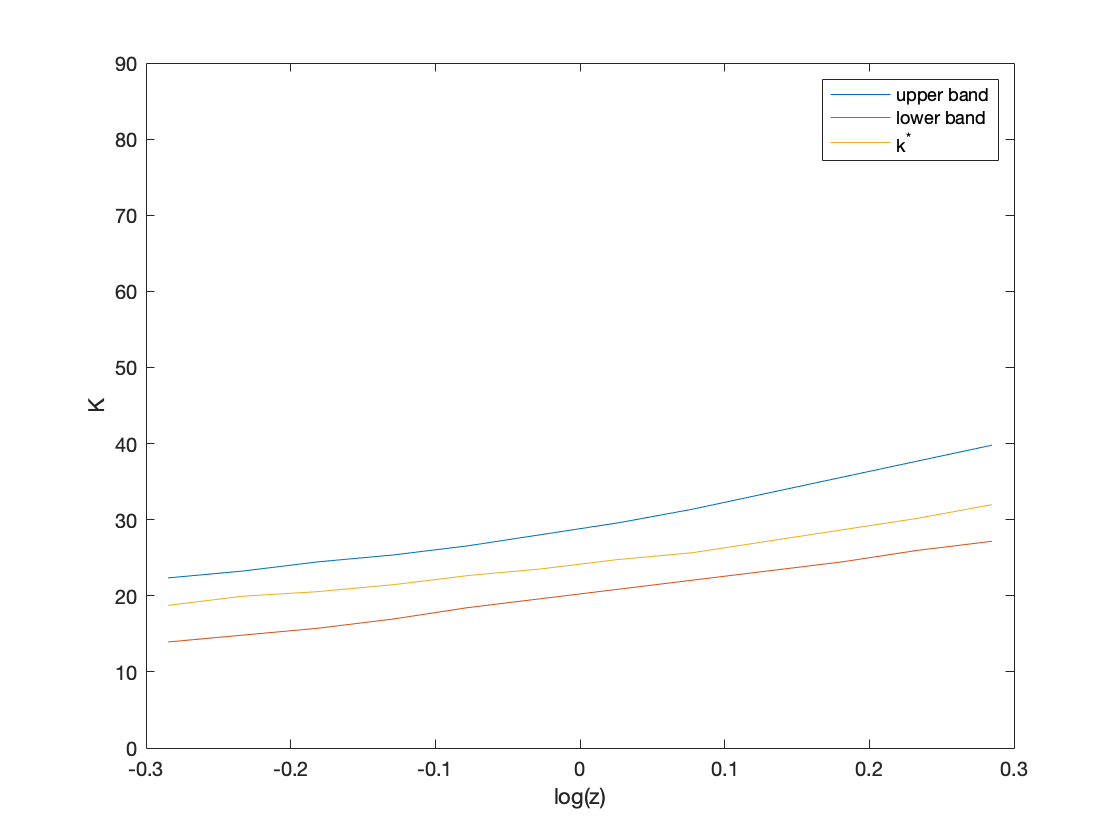
\includegraphics[width=8cm]{ps3q2_fig1}
\caption{Bands for (i) a}
\end{subfigure}
\begin{subfigure}{.5\textwidth}
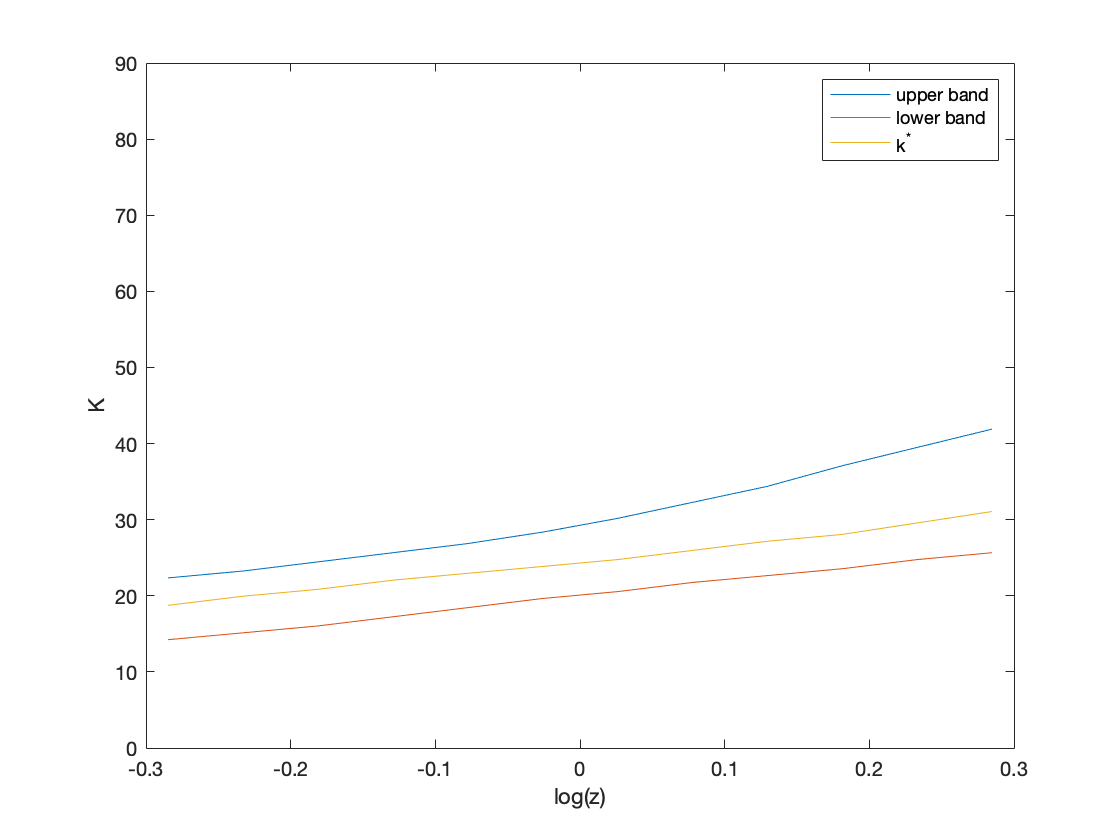
\includegraphics[width=8cm]{ps3q2_fig2}
\caption{Bands for (i) b}
\end{subfigure}
\begin{subfigure}{.5\textwidth}
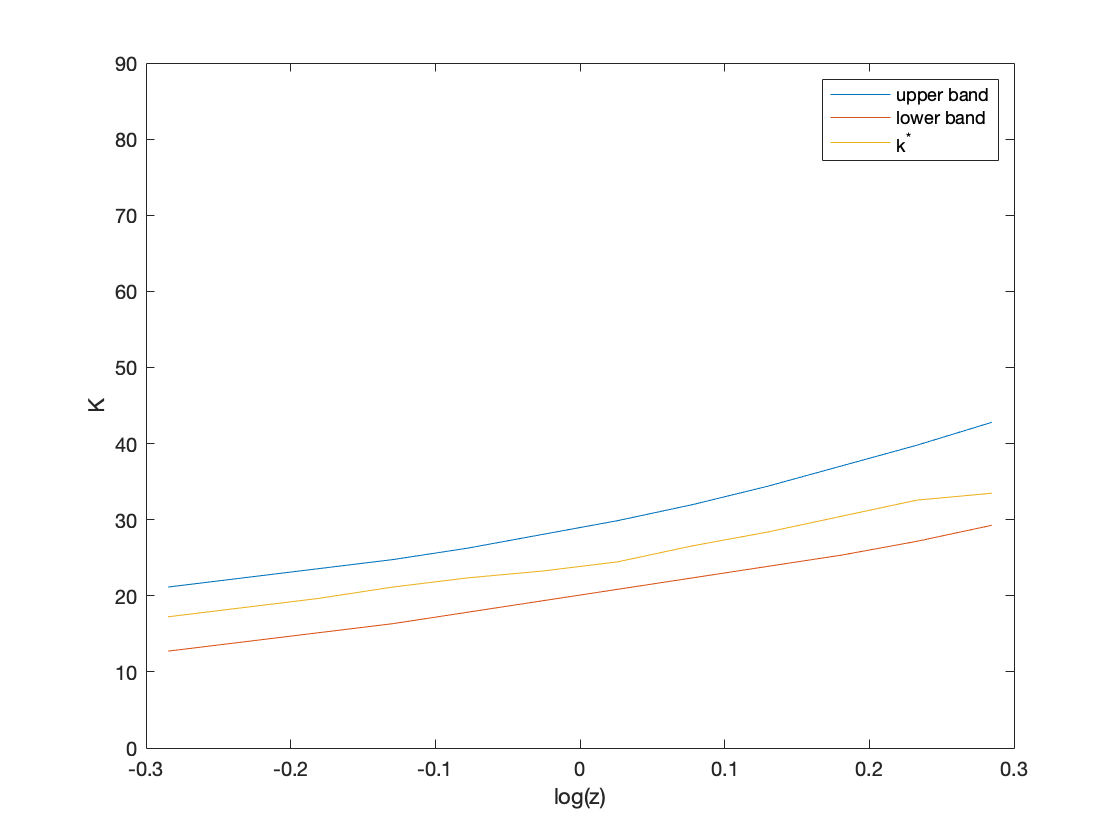
\includegraphics[width=8cm]{ps3q2_fig3}
\caption{Bands for (ii) a}
\end{subfigure}
\begin{subfigure}{.5\textwidth}
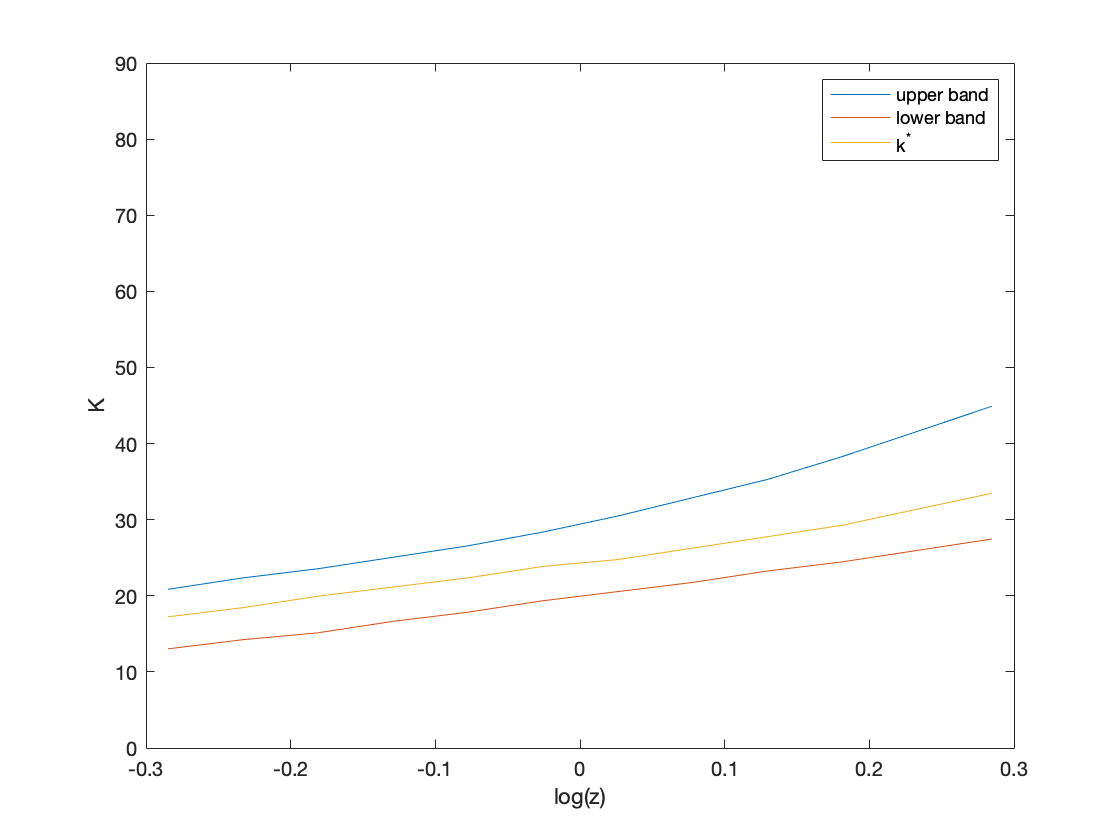
\includegraphics[width=8cm]{ps3q2_fig4}
\caption{Bands for (ii) b}
\end{subfigure}
\caption{Benchmark cases}
\end{figure}
\end{center}
\problempart{(4)}
In case (i)a, the bands are constant over $z$, since $z$ is iid drawn over time, and the slope remains fixed and the width is fixed. In (i)b, the bands surround the same $k^*$ (since $z$ is iid), but the width increases since more productive firms pay a higher cost to adjust. In (ii), the slope is increasing due to the effect of productivity on the current value of capital. The band is wider around the extreme values of $z$, since more productive firms are willing to keep higher levels of capital for larger profits in the current period, where less productive firms maintain low levels of capital to avoid losses in the current period.
\begin{center}
\begin{figure}
\begin{subfigure}{.5\textwidth}
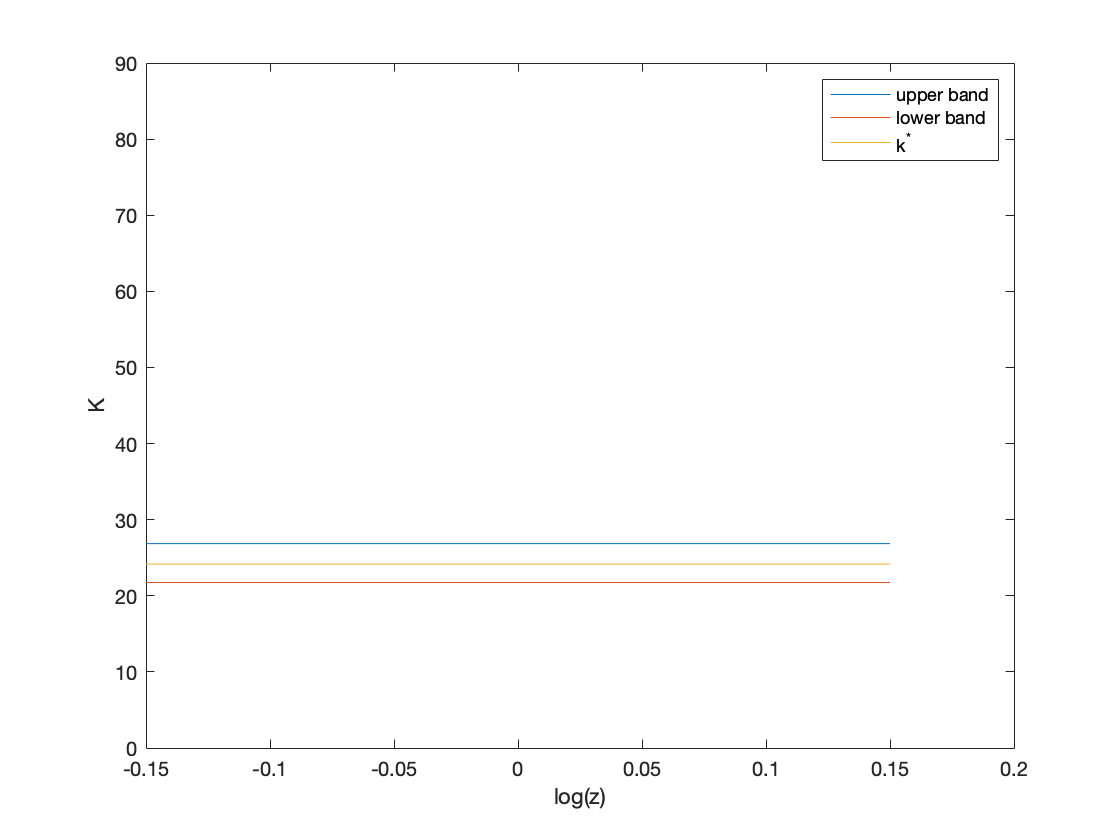
\includegraphics[width=8cm]{ps3q2_fig5}
\caption{Bands for (i) a}
\end{subfigure}
\begin{subfigure}{.5\textwidth}
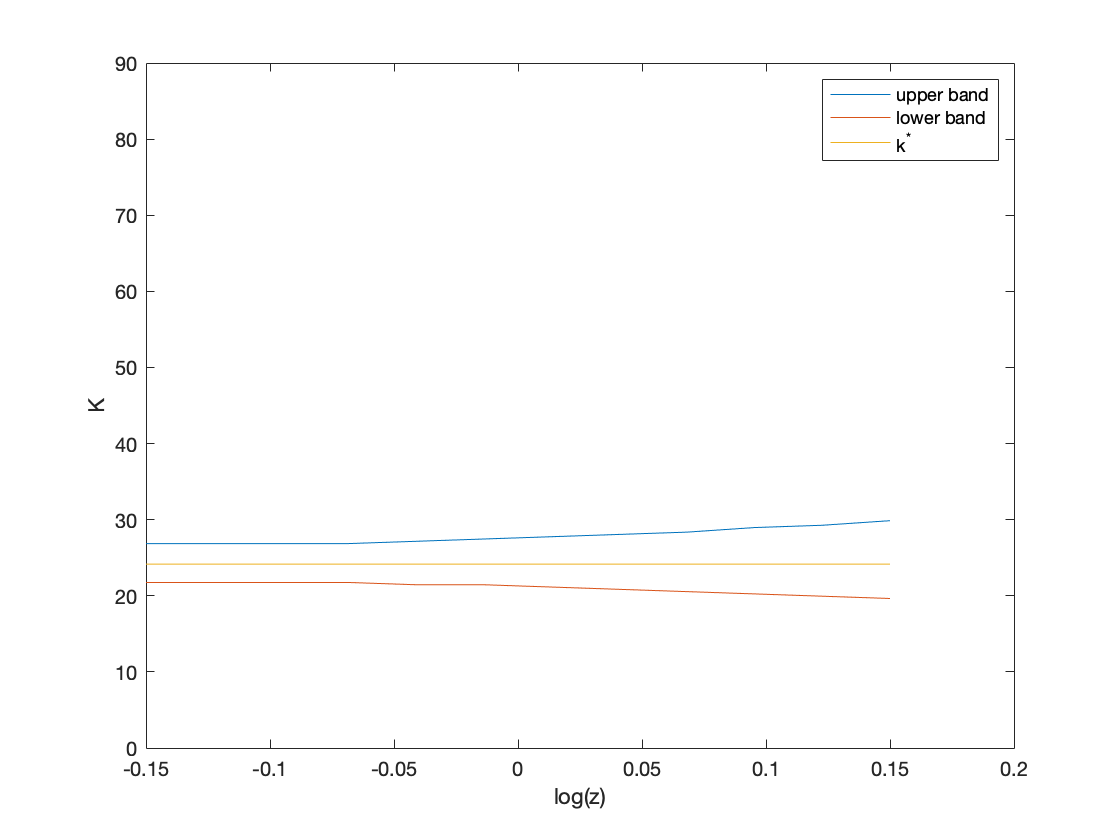
\includegraphics[width=8cm]{ps3q2_fig6}
\caption{Bands for (i) b}
\end{subfigure}
\begin{subfigure}{.5\textwidth}
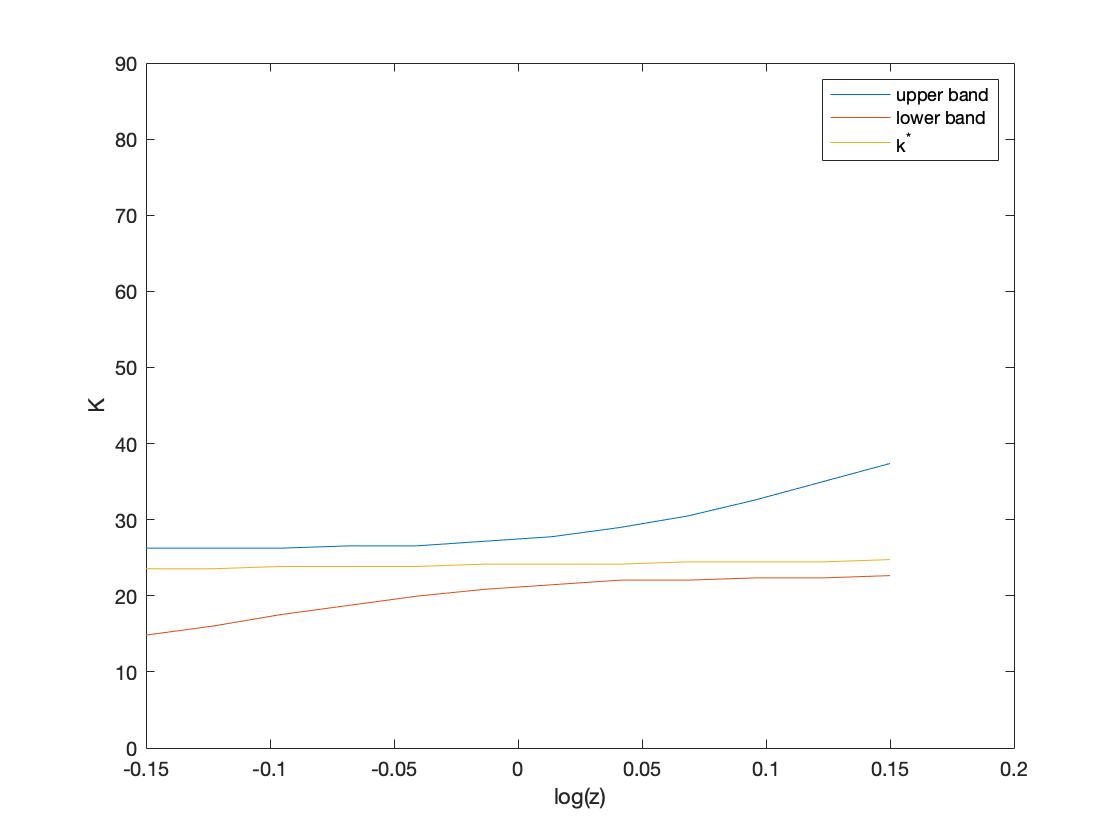
\includegraphics[width=8cm]{ps3q2_fig7}
\caption{Bands for (ii) a}
\end{subfigure}
\begin{subfigure}{.5\textwidth}
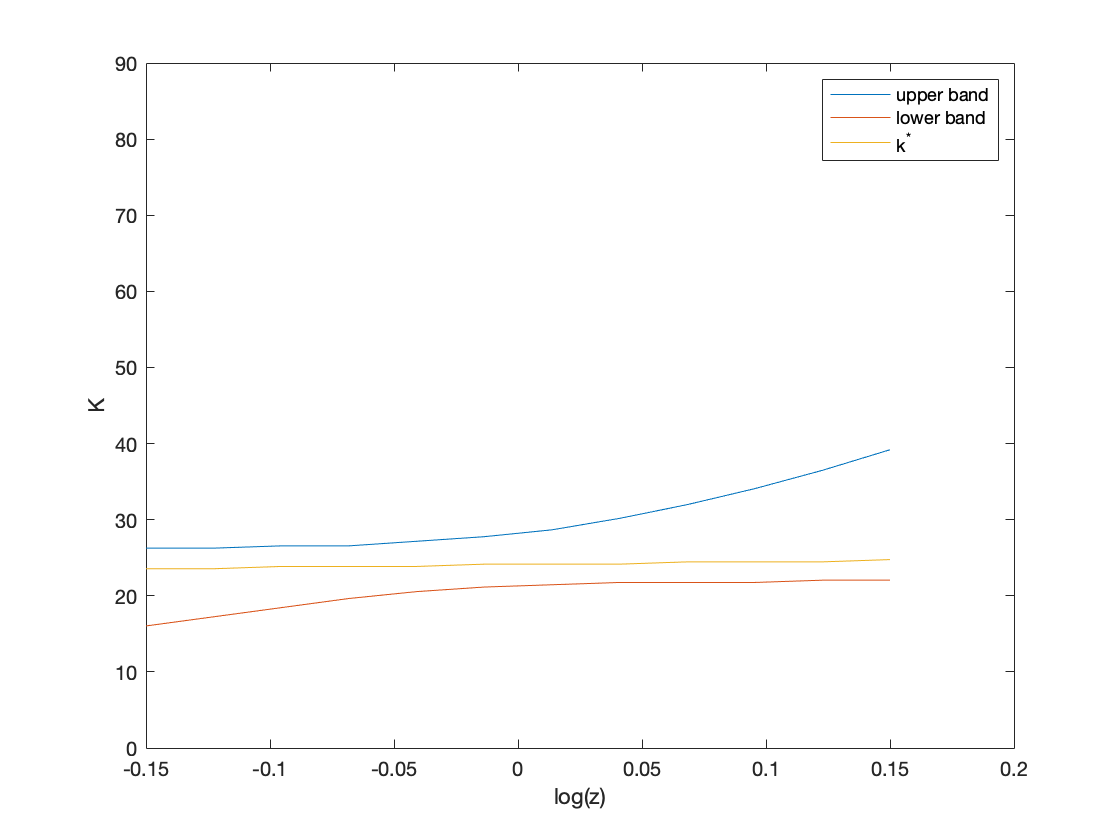
\includegraphics[width=8cm]{ps3q2_fig8}
\caption{Bands for (ii) b}
\end{subfigure}
\caption{$\rho = 0$ cases}
\end{figure}
\end{center}
\problempart{(5)} The larger adjustment cost increases the width of the inaction bands; the larger the costs, the more tolerant you will be of being farther away from $k^*$.
\begin{center}
\begin{figure}
\begin{subfigure}{.5\textwidth}
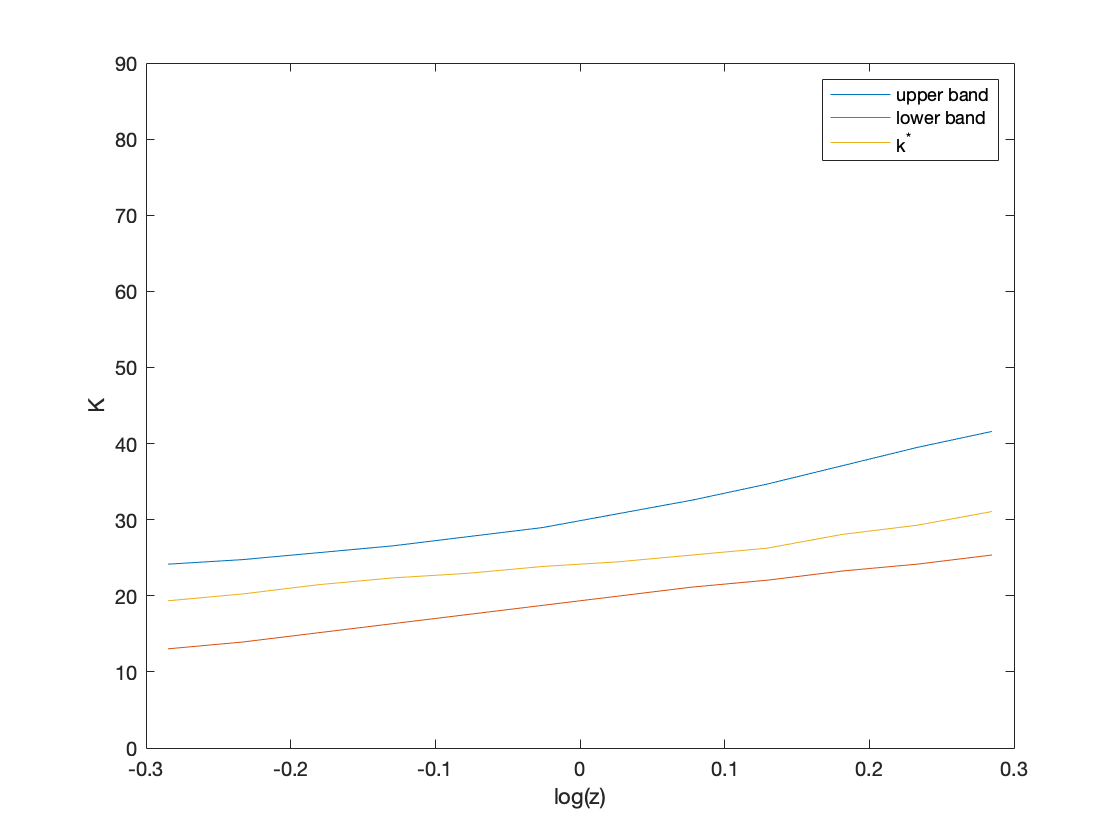
\includegraphics[width=8cm]{ps3q2_fig9}
\caption{Bands for (i) a}
\end{subfigure}
\begin{subfigure}{.5\textwidth}
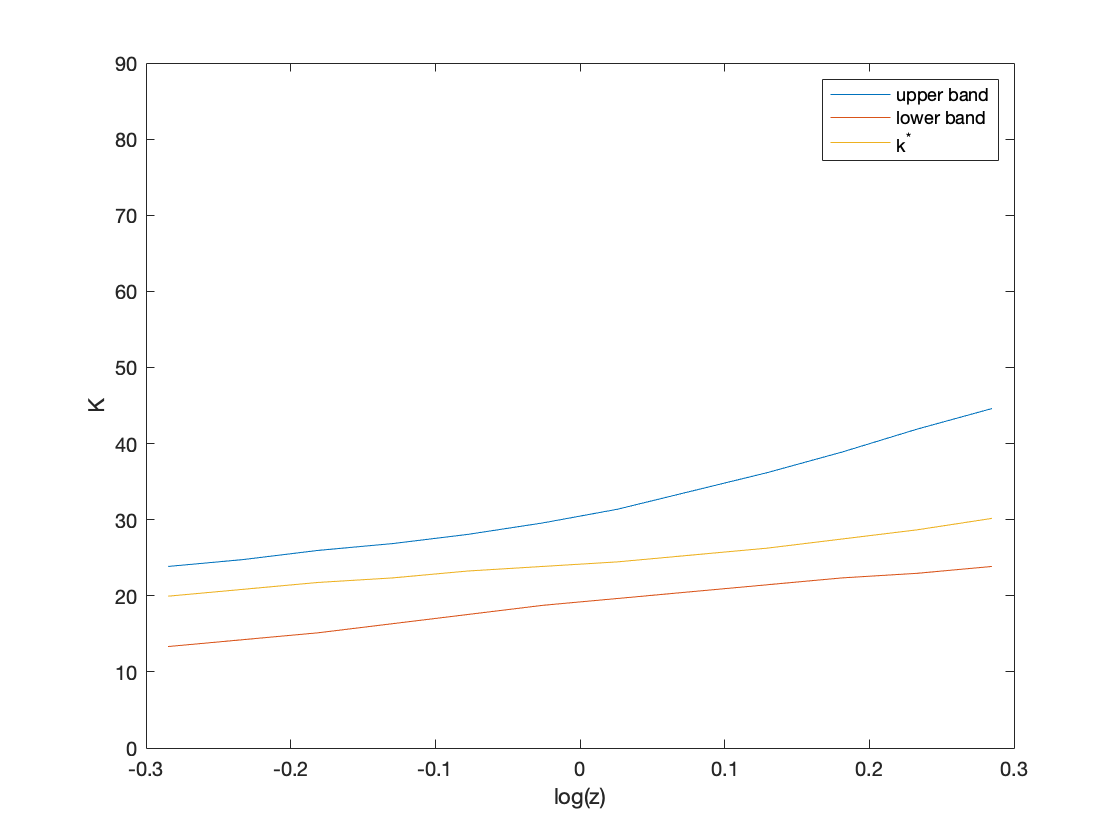
\includegraphics[width=8cm]{ps3q2_fig10}
\caption{Bands for (i) b}
\end{subfigure}
\begin{subfigure}{.5\textwidth}
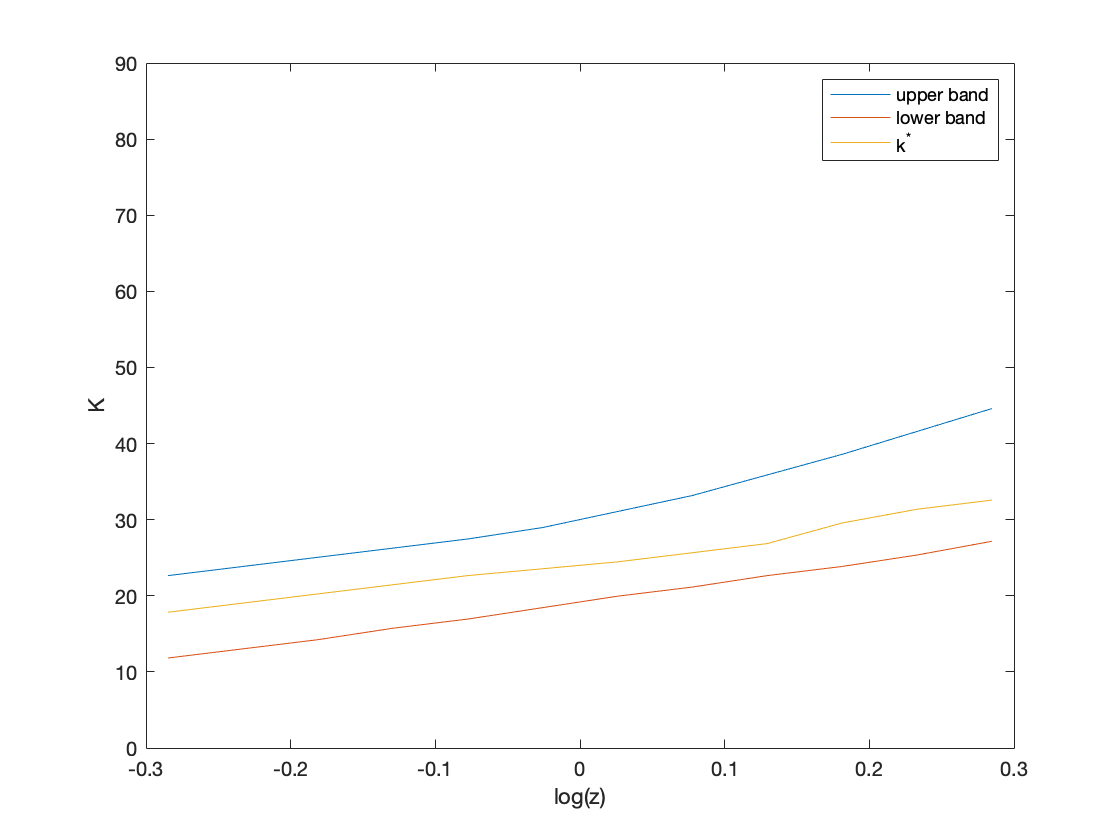
\includegraphics[width=8cm]{ps3q2_fig11}
\caption{Bands for (ii) a}
\end{subfigure}
\begin{subfigure}{.5\textwidth}
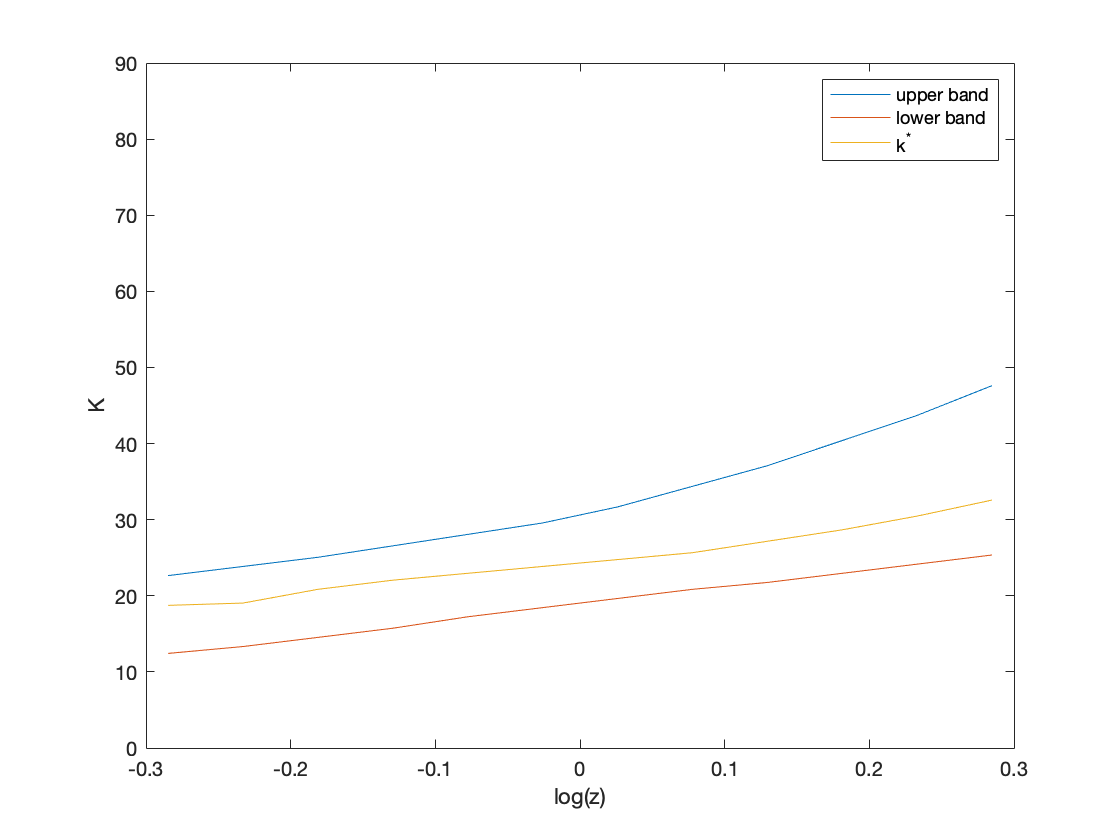
\includegraphics[width=8cm]{ps3q2_fig12}
\caption{Bands for (ii) b}
\end{subfigure}
\caption{Doubled adjustment costs}
\end{figure}
\end{center}
\problempart{(6)} Increasing $\sigma$ makes all the slopes steeper in all cases, due to convexity of the profit function in $\log z$. Larger variance disproportionately yields more profits from high tails than losses from low tails. The width also increases in all cases since firms are more willing to accept waiting for the next period since the shock is more variable. We expect frequency of adjustments to decrease in this case.
\begin{center}
\begin{figure}
\begin{subfigure}{.5\textwidth}
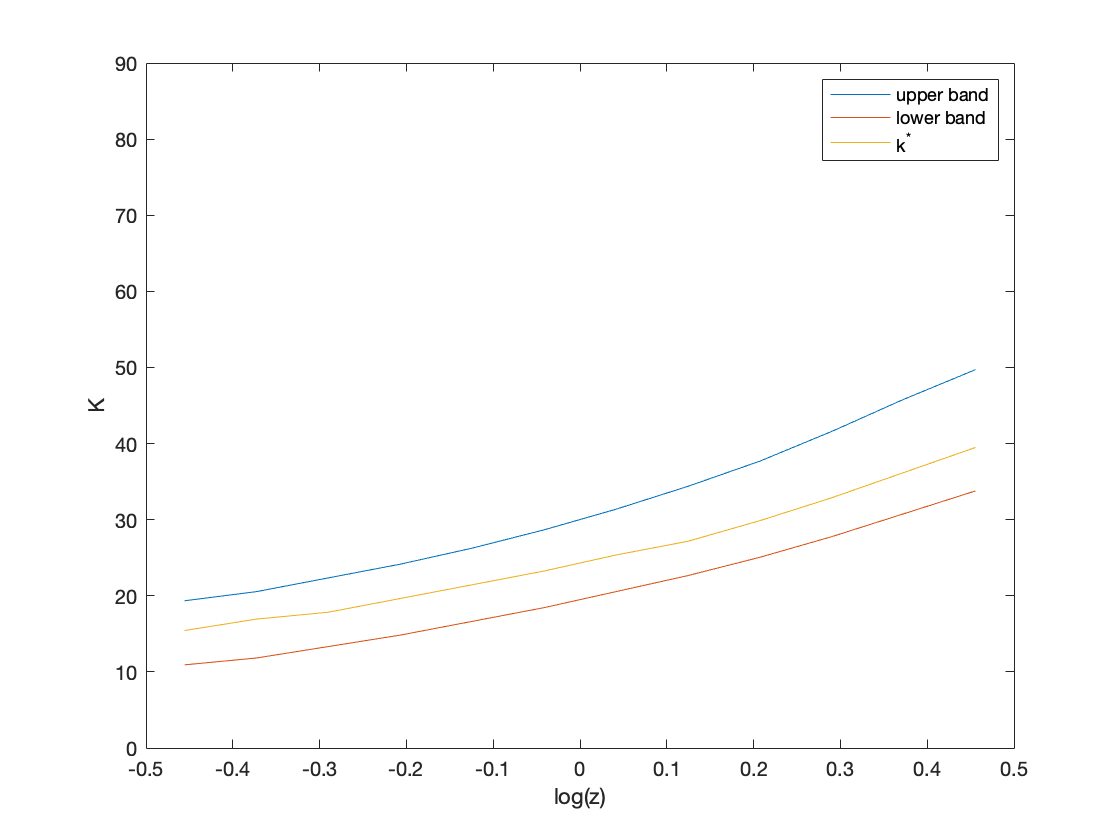
\includegraphics[width=8cm]{ps3q2_fig13}
\caption{Bands for (i) a}
\end{subfigure}
\begin{subfigure}{.5\textwidth}
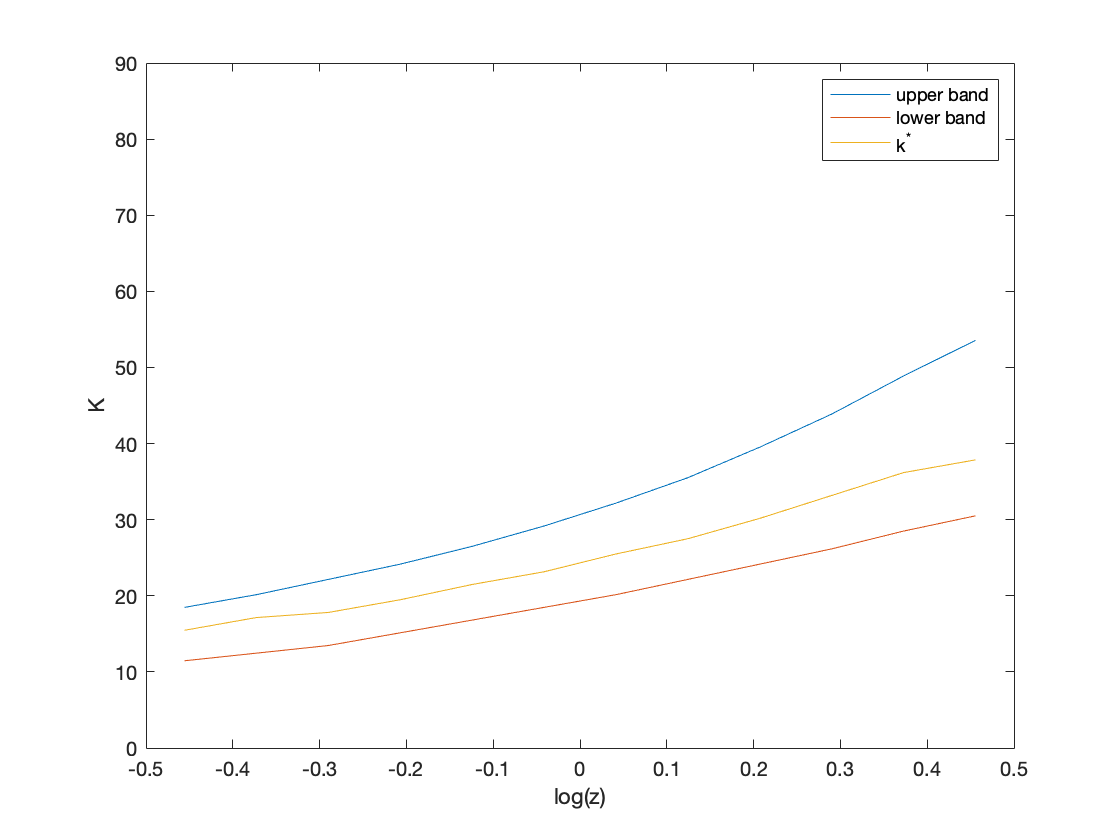
\includegraphics[width=8cm]{ps3q2_fig14}
\caption{Bands for (i) b}
\end{subfigure}
\begin{subfigure}{.5\textwidth}
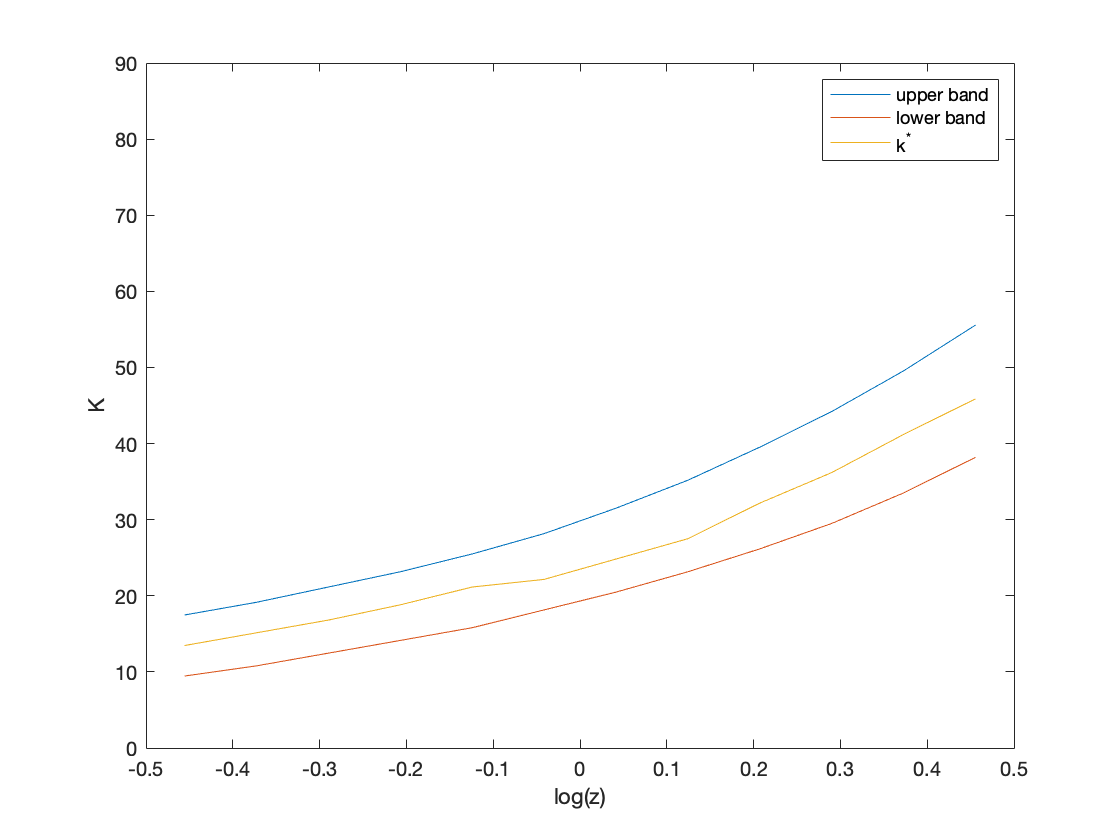
\includegraphics[width=8cm]{ps3q2_fig15}
\caption{Bands for (ii) a}
\end{subfigure}
\begin{subfigure}{.5\textwidth}
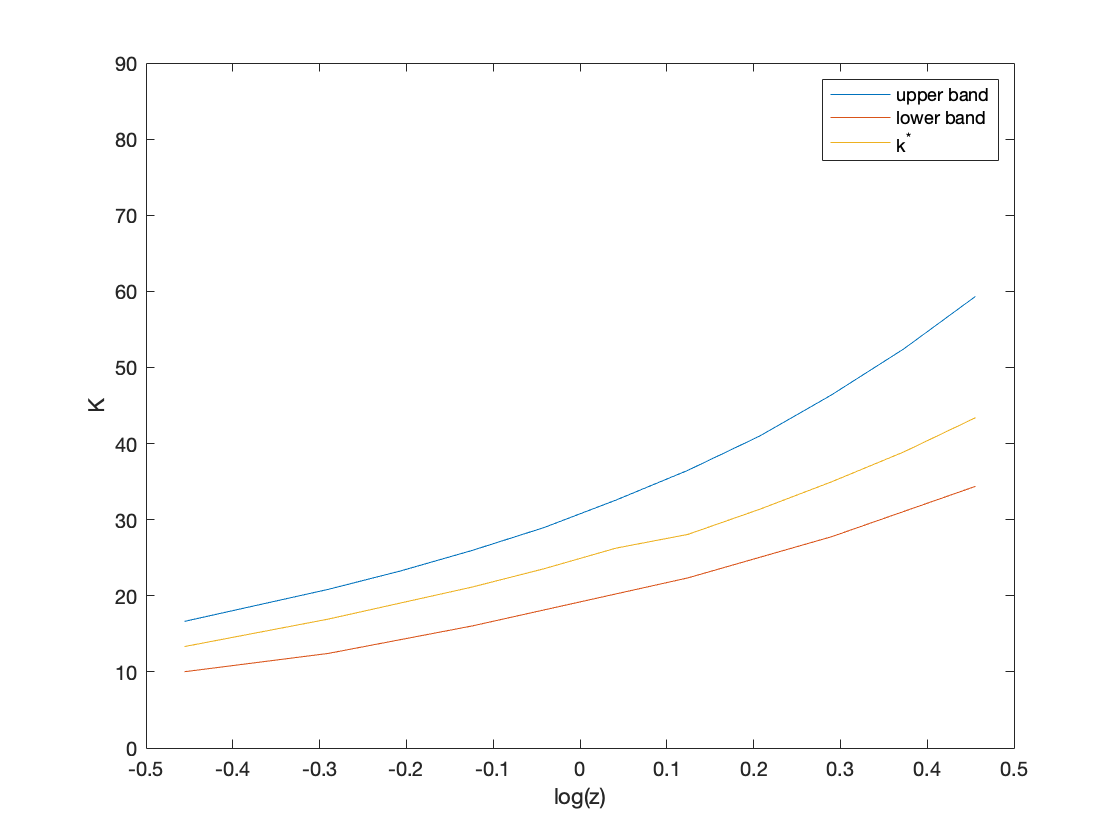
\includegraphics[width=8cm]{ps3q2_fig16}
\caption{Bands for (ii) b}
\end{subfigure}
\caption{Increased $\sigma$}
\end{figure}
\end{center}
\problempart{(7)} The widening as a result of increasing $\sigma$ is smaller for larger $\delta$. When $\delta$ is large, the option to wait for a more / less productive period to adjust capital is much more costly, and hence the width of the inaction band decreases and is less sensitive to $\sigma$.
\begin{center}
\begin{figure}
\begin{subfigure}{.5\textwidth}
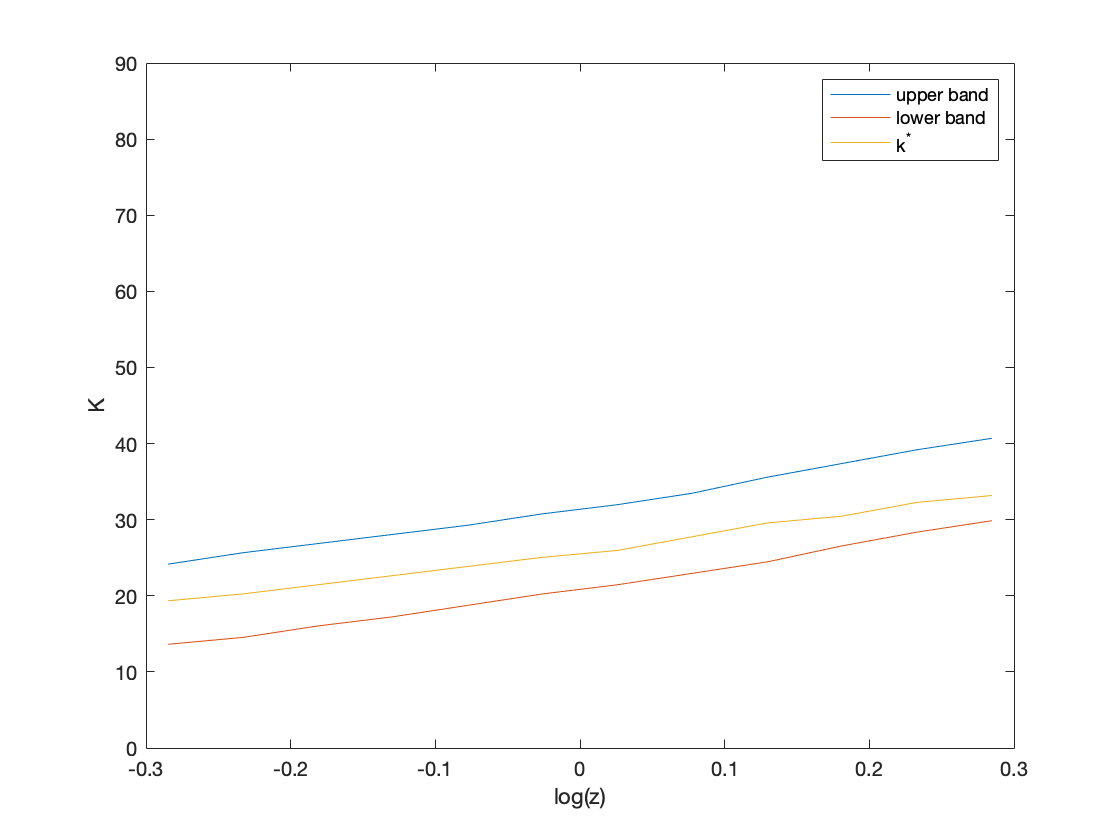
\includegraphics[width=8cm]{ps3q2_fig17}
\caption{Bands for (i) a}
\end{subfigure}
\begin{subfigure}{.5\textwidth}
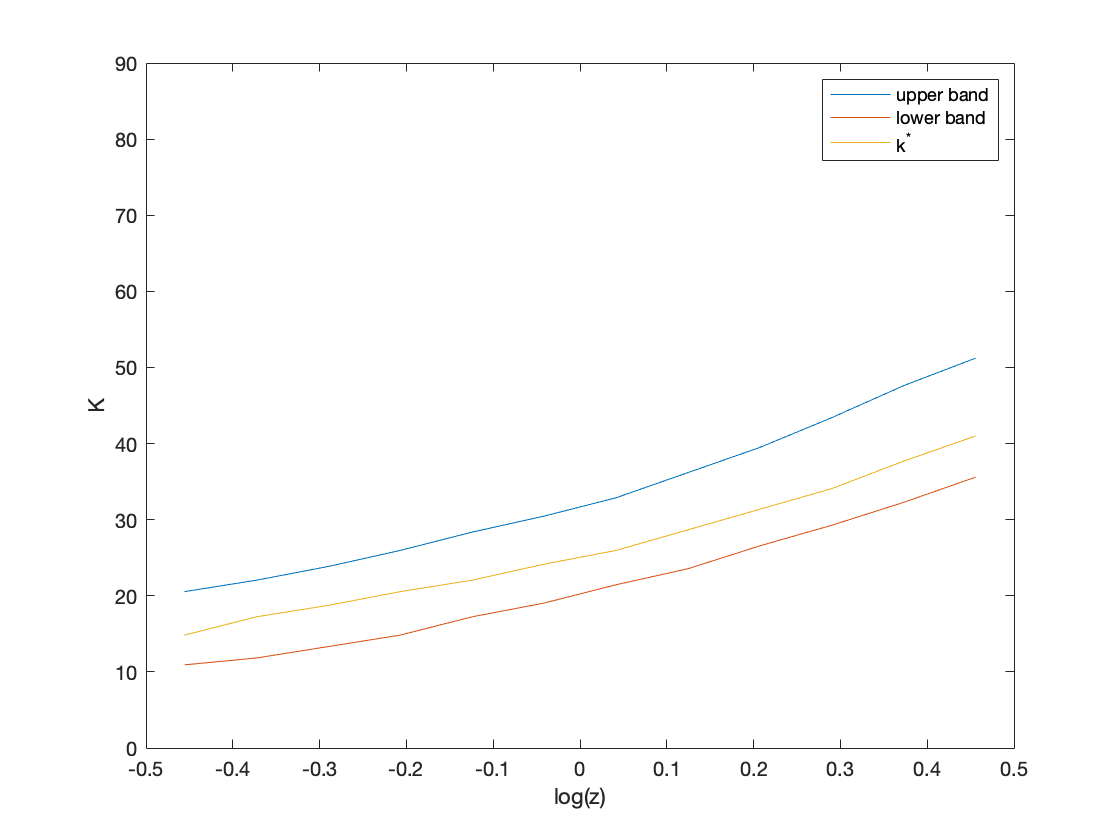
\includegraphics[width=8cm]{ps3q2_fig18}
\caption{Bands for (i) a, increased $\sigma$}
\end{subfigure}
\begin{subfigure}{.5\textwidth}
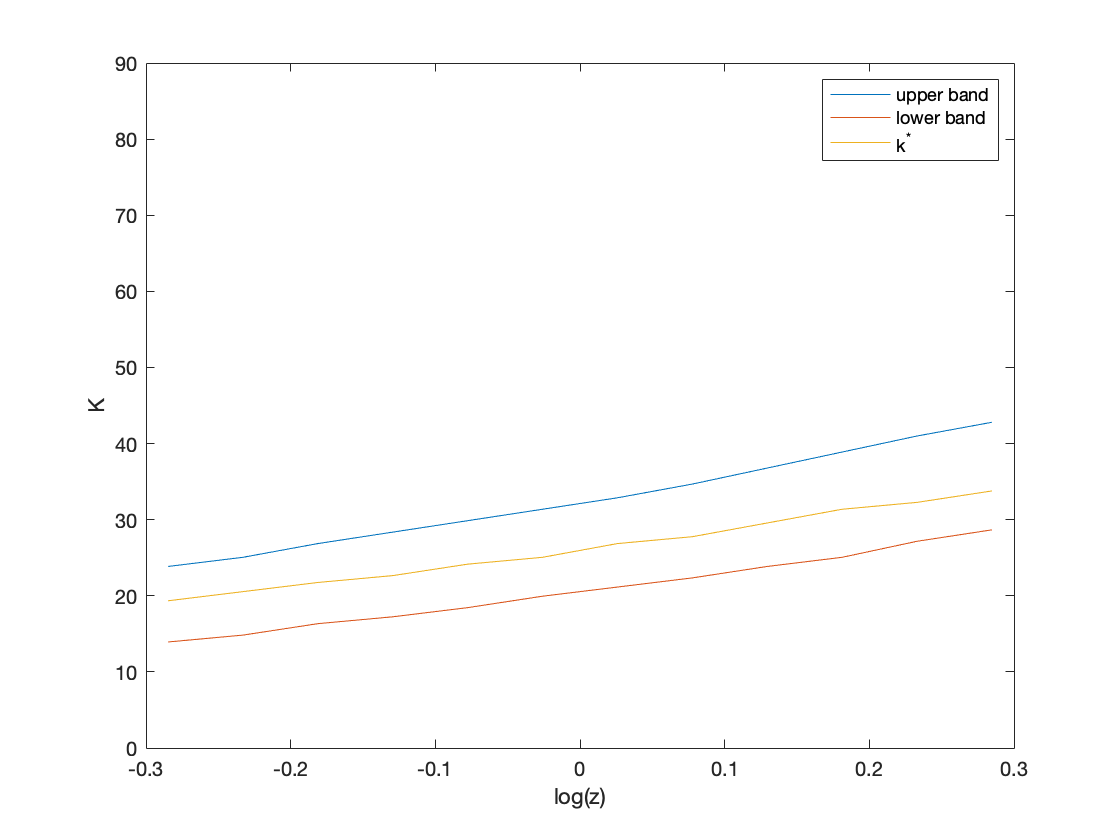
\includegraphics[width=8cm]{ps3q2_fig19}
\caption{Bands for (i) b}
\end{subfigure}
\begin{subfigure}{.5\textwidth}
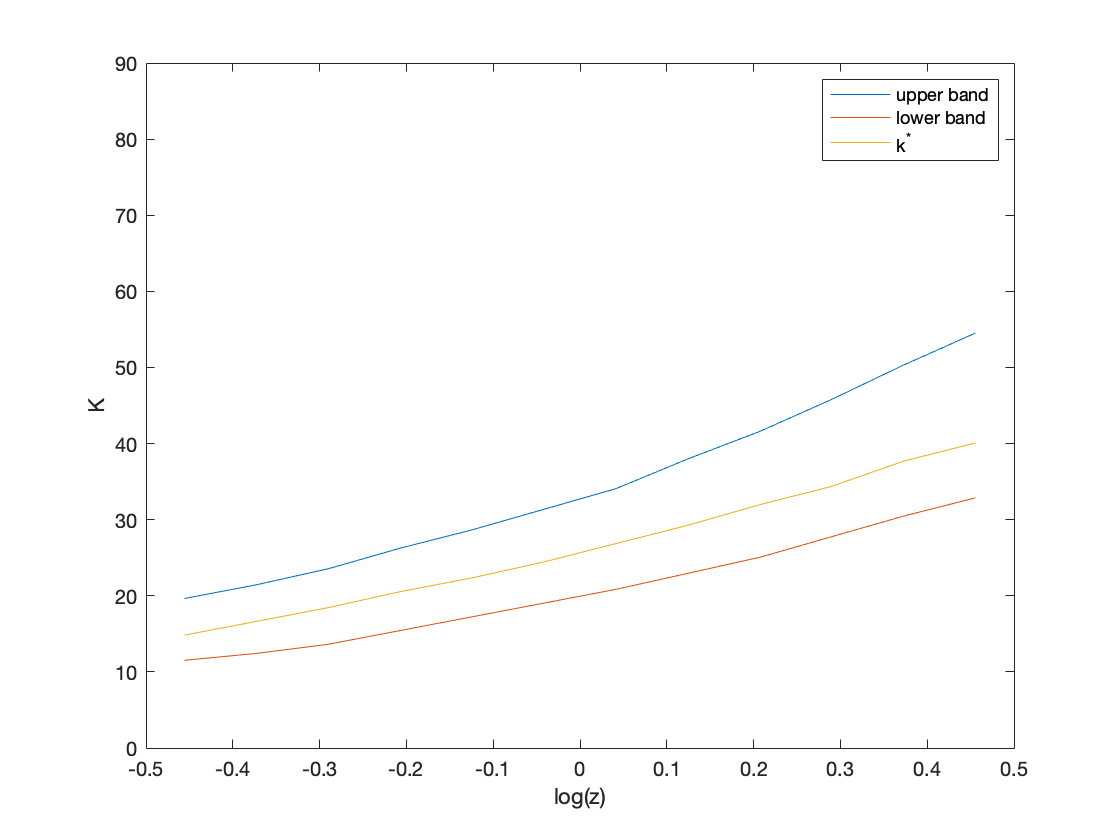
\includegraphics[width=8cm]{ps3q2_fig20}
\caption{Bands for (i) b, increased $\sigma$}
\end{subfigure}
\caption{Increased $\delta$, model (i)}
\end{figure}
\begin{figure}
\begin{subfigure}{.5\textwidth}
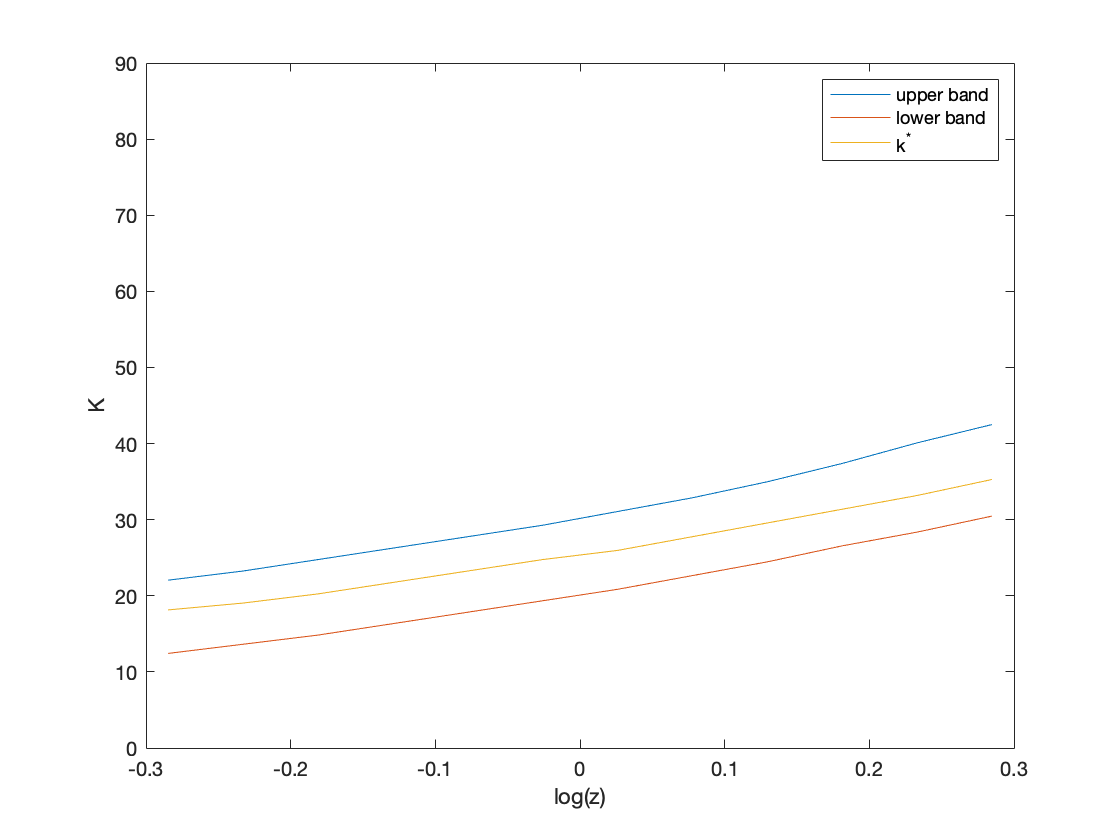
\includegraphics[width=8cm]{ps3q2_fig21}
\caption{Bands for (ii) a}
\end{subfigure}
\begin{subfigure}{.5\textwidth}
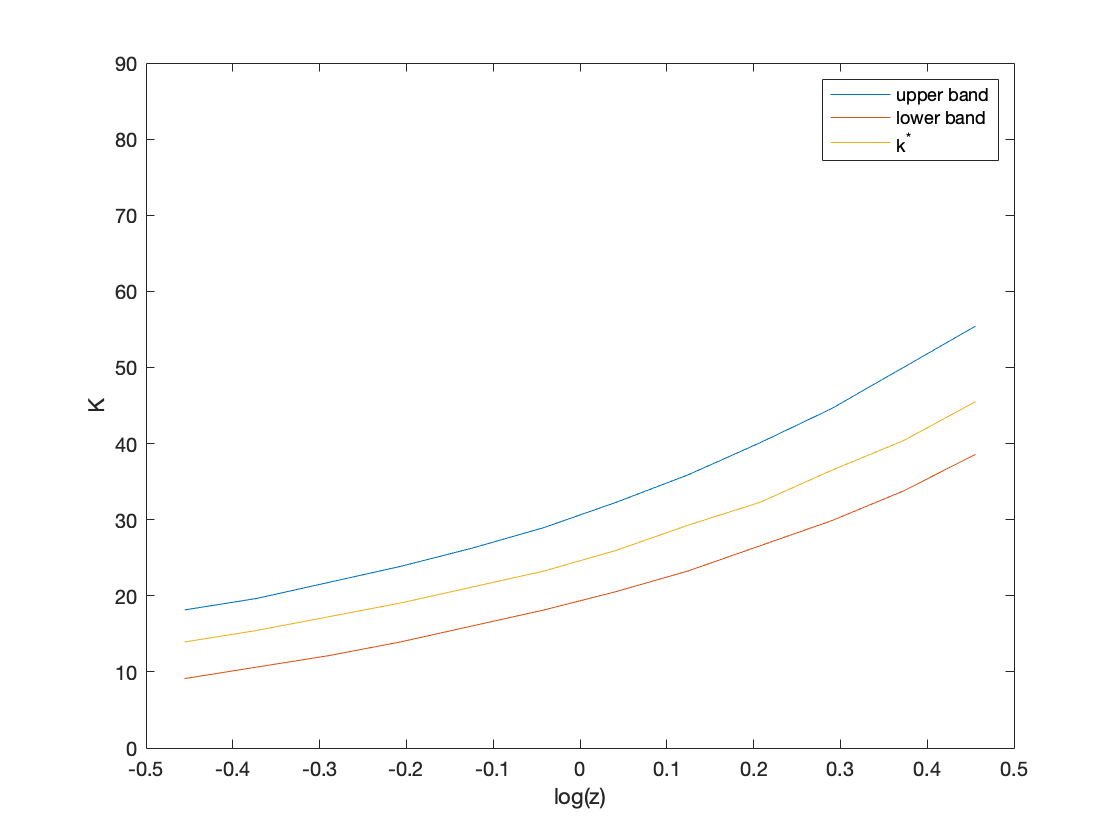
\includegraphics[width=8cm]{ps3q2_fig22}
\caption{Bands for (ii) a, increased $\sigma$}
\end{subfigure}
\begin{subfigure}{.5\textwidth}
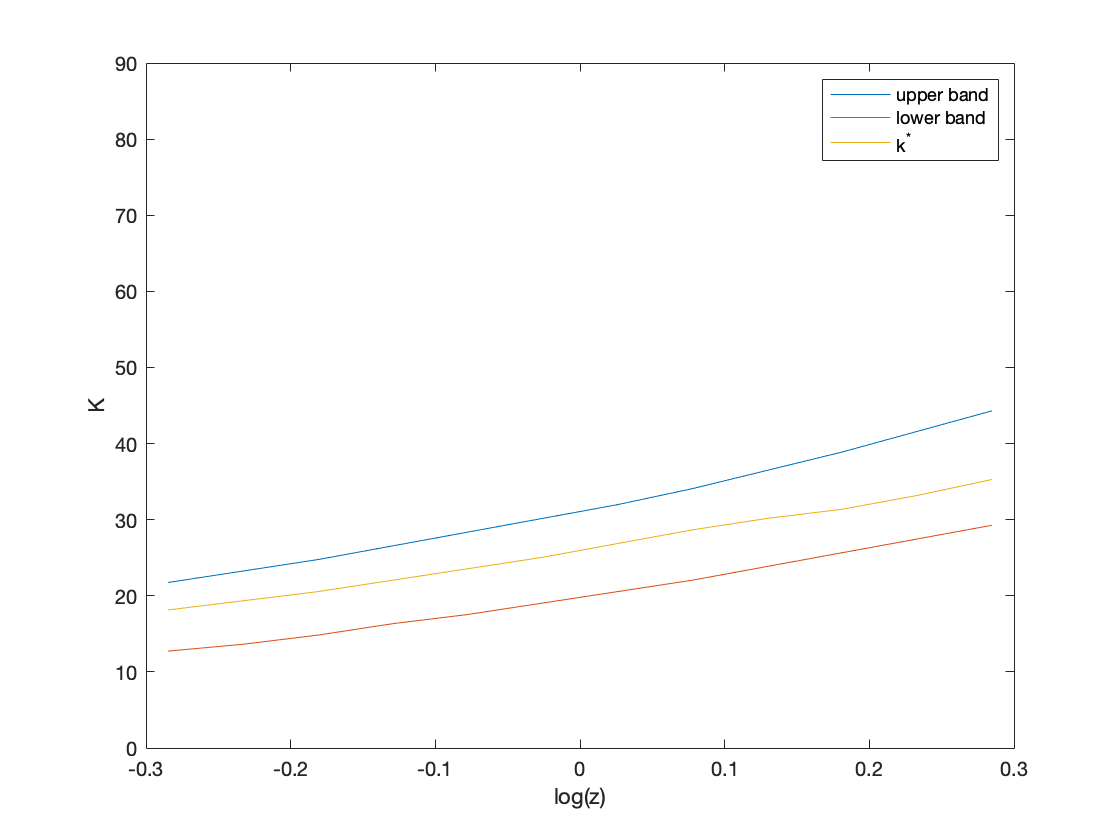
\includegraphics[width=8cm]{ps3q2_fig23}
\caption{Bands for (ii) b}
\end{subfigure}
\begin{subfigure}{.5\textwidth}
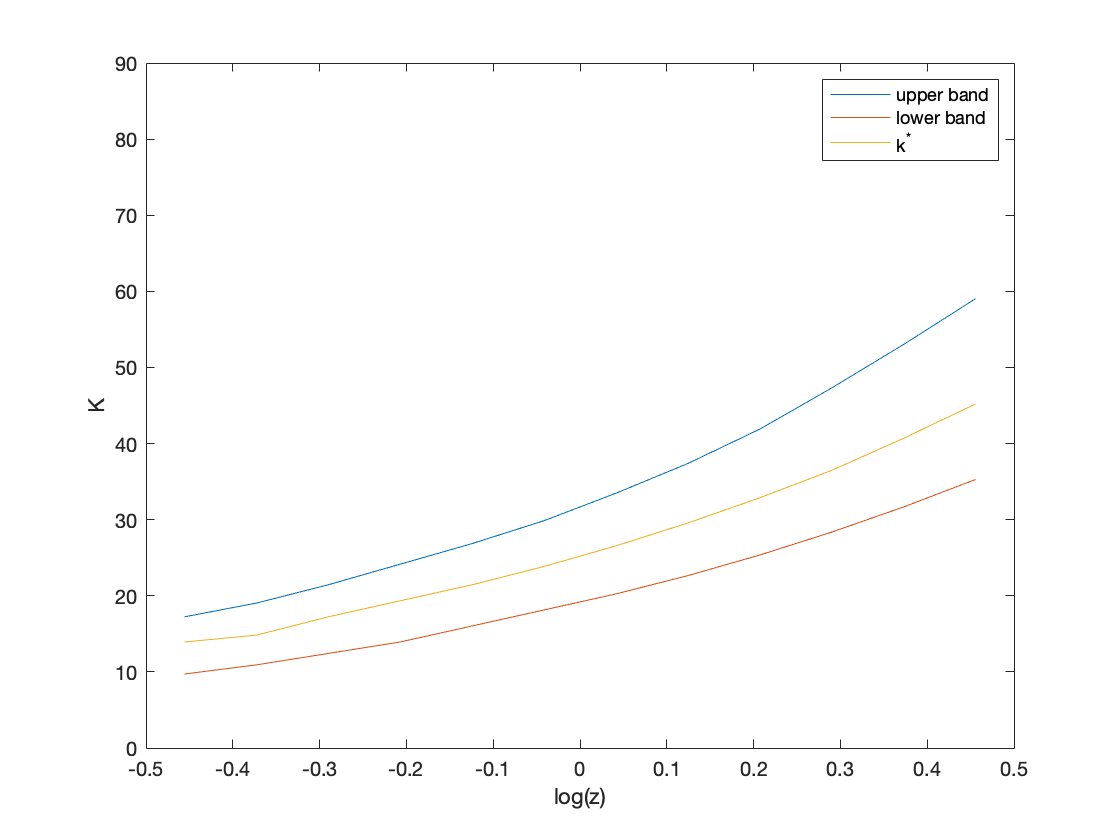
\includegraphics[width=8cm]{ps3q2_fig24}
\caption{Bands for (ii) b, increased $\sigma$}
\end{subfigure}
\caption{Increased $\delta$, model (ii)}
\end{figure}
\end{center}
\end{document}
	% line of code telling latex that your document is ending. If you leave this out, you'll get an error
